\section{後処理と描画} \label{sec:ideal_exp_net2g}
%------------------------------------------------------
ここでは、後処理と計算結果の描画方法について説明する。本書のチュートリアルでは、
NetCDF形式の分散ファイルを1つのファイルにまとめ、ダイレクトアクセスが可能な
単純バイナリ形式(\grads 形式)に変換する方法を説明する。
このバイナリ形式は、ユーザーによる結果の解析を容易にする。
%GPhys/Ruby-DCLを使うと
%分割ファイルのまま直接描画することができるが、この方法については\ref{sec:quicklook}節を
%参照してもらいたい。

まず、\ref{sec:source_net2g}節でコンパイルした後処理ツール\verb|net2g|へリンクを張る。
\begin{verbatim}
  $ ln -s ../../../util/netcdf2grads_h/net2g  ./
\end{verbatim}
%もし、ここで説明するディレクトリとは異なる場所で実行している場合は、
%リンクを張る時のディレクトリ指定に注意すること。

\verb|net2g| の実行方法は、基本的に{\scalerm}と同じであり、
\begin{verbatim}
  $ mpirun  -n  [プロセス数]  ./net2g  [設定ファイル]
\end{verbatim}
の形式で実行する。
net2g専用の \verb|net2g_R20kmDX500m.conf|を設定ファイルとして与えて、
次のように実行する。
\begin{verbatim}
  $ mpirun  -n  2  ./net2g  net2g_R20kmDX500m.conf
\end{verbatim}
エラーメッセージがなく、下記のメッセージだけが標準出力へ表示されていれば、正常に変換は完了している。\\

\noindent {\gt
\fbox{
\begin{tabularx}{150mm}{l}
\verb|+++ MPI COMM: Corrective Finalize| \\
\end{tabularx}
}}\\

\noindent net2gの実行には、{\scalerm}の実行時に使用したMPIプロセス数と同じか、
その約数のプロセス数を使用しなければならない。
%HDDの読み書き速度に依存するが、本書の必要要件にあった計算機であれば2分程度で計算が終わる。
この実行によって、実行ディレクトリ下に下記6つのファイルが作成される。
\begin{alltt}
  QHYD_d01z-3d.ctl
  QHYD_d01z-3d.grd
  U_d01z-3d.ctl
  U_d01z-3d.grd
  W_d01z-3d.ctl
  W_d01z-3d.grd
\end{alltt}
「grd」ファイルは、分割ファイルを結合することによって得られる、
ダイレクトアクセス可能の単純バイナリ形式(\grads 形式)である。
一方、「ctl」ファイルは、\grads によって「grd」ファイルを読む込むときに必要な情報を含む。

計算が問題なく完了しているかを確認するため、\grads スクリプト \verb|checkfig_ideal.gs|
を使って作図する。なお、\grads のバージョンによって文法が異なるため、
警告が出る場合には\grads スクリプトを適宜変更されたい。
\begin{verbatim}
  $ grads -blc checkfig_ideal.gs
\end{verbatim}
作図が成功すると、下記の図が生成される。
\begin{verbatim}
   ideal_QHYD.png
   ideal_W.png
\end{verbatim}
シミュレーションと後処理が成功していれば、図\ref{fig_ideal}と同じ図が得られる。

\begin{figure}[t]
\begin{center}
  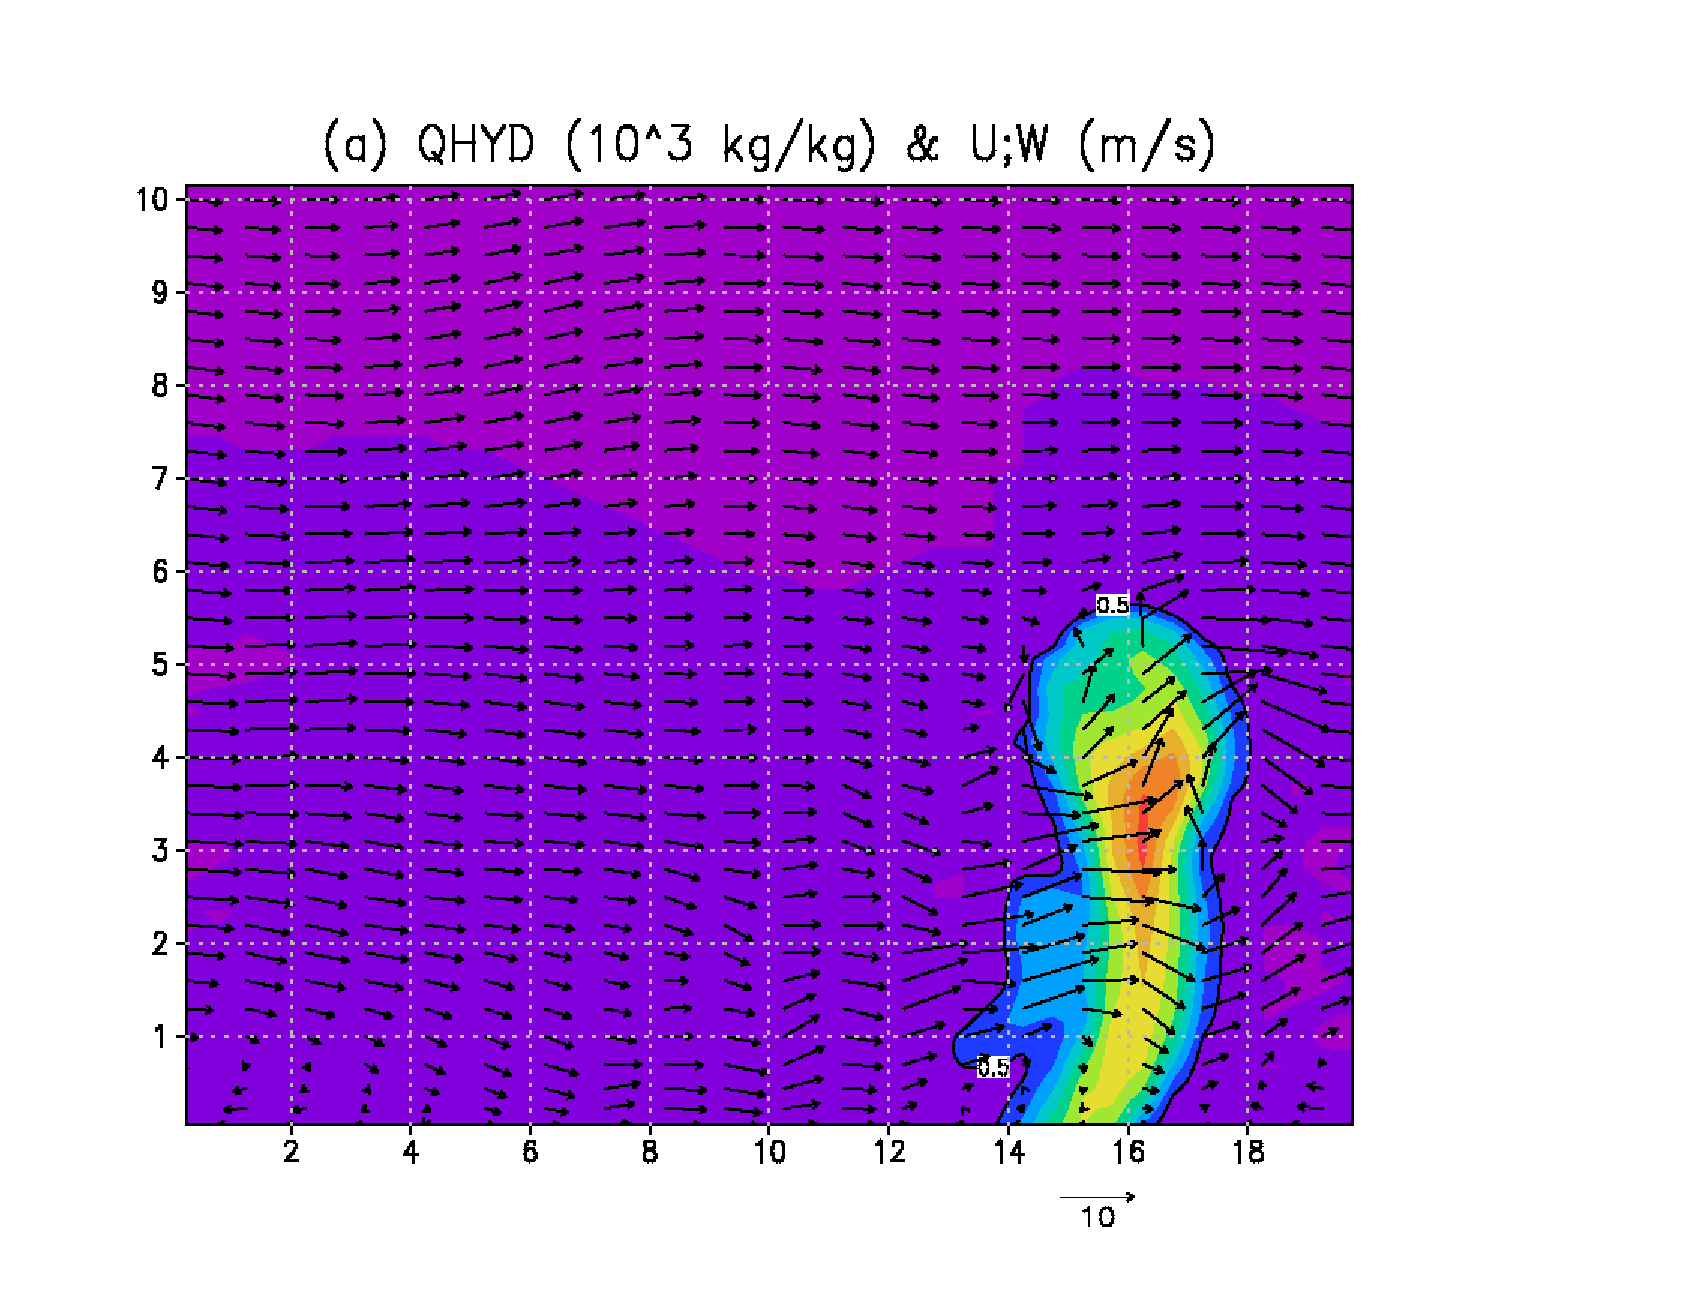
\includegraphics[width=0.7\hsize]{./figure/ideal_qhyd.eps}\\
  \includegraphics[width=0.7\hsize]{./figure/ideal_W.eps}\\
  \caption{積分開始から 1200 秒(20 分)後の Y=750 mにおける東西-鉛直断面図;
           カラーシェードは、(a)において全質量に対する凝結物の質量比、
           (b)において鉛直速度を表す。ベクトルは東西-鉛直断面内の風の流れを表す。}
  \label{fig_ideal}
\end{center}
\end{figure}


他の変数についてもバイナリデータに変換したい場合には、
\verb|net2g_R20kmDX500m.conf|の\namelist{VARI}の\nmitem{VNAME} に必要な変数を追加すればよい。\\

\noindent {\small {\gt
\ovalbox{
\begin{tabularx}{150mm}{l}
\verb|&VARI|\\
\verb| VNAME       = "U","W","QHYD"|\\
\verb|/|\\
\end{tabularx}
}}}\\

\noindent
historyファイルに出力されている変数は、{\netcdf} の\verb|ncdump| などを
使えば簡単に確認できる。net2gの詳しい使用方法は、第\ref{sec:net2g}節を参照されたい。




